% Fisica Computacional (106018C) - Taller 7, Semana 7
% Cristian Andres Cardenas Munoz - 2518531
% Reporte de una sola pagina; acompanado por codigo y datos reproducibles.
\documentclass[10pt,a4paper]{article}
\usepackage[spanish,es-noshorthands]{babel}
\usepackage[T1]{fontenc}
\usepackage[utf8]{inputenc}
\usepackage{lmodern}
\usepackage[a4paper,margin=1.78cm,top=1.6cm,bottom=1.55cm]{geometry}
\usepackage{amsmath,amssymb}
\usepackage{booktabs}
\usepackage{graphicx}
\usepackage{hyperref}
\hypersetup{colorlinks=true,urlcolor=black,linkcolor=black}
\pagestyle{empty}
\setlength{\parindent}{0pt}
\setlength{\parskip}{4pt}
\setlength{\abovedisplayskip}{4pt}
\setlength{\belowdisplayskip}{4pt}
\begin{document}
\begin{center}
{\large\bfseries Física Computacional (106018C)}\\[2pt]
{\bfseries Taller 7 --- Integración y derivación numérica}\\[2pt]
Semana 7 --- Fortran y Python\\[2pt]
Cristian Andrés Cárdenas Muñoz (2518531) --- 12/11/2026
\end{center}
\vspace{1pt}\hrule\vspace{5pt}

\textbf{1. Contexto físico.}
Se estudió un oscilador amortiguado, $x(t)=e^{-0.5t}\cos(2\pi t)$, cuya energía mecánica disminuye por la fricción. Se calcularon la energía disipada en tres segundos y las derivadas de la posición muestreada. La identidad $\int_0^3 2\gamma v(t)^2\,dt=E(0)-E(3)$ proporciona una referencia independiente para comprobar el cálculo.

\textbf{2. Método.}
En Fortran se implementó integración de Romberg con trapecios refinados y extrapolación de Richardson, tabla \texttt{allocatable} desde índice cero y evaluación exclusiva de puntos nuevos. En Python se usaron rebanadas de NumPy para derivadas adelantada, atrasada, central, de cinco puntos y segunda derivada central (sin funciones de derivación de bibliotecas):
\[
 S_{k,j}=\frac{4^jS_{k,j-1}-S_{k-1,j-1}}{4^j-1},\qquad
 v_i\simeq\frac{x_{i+1}-x_{i-1}}{2\Delta t},\qquad
 a_i\simeq\frac{x_{i+1}-2x_i+x_{i-1}}{\Delta t^2}.
\]

\textbf{3. Resultados e interpretación.}
El balance energético dio $E_{\mathrm{dis}}=18.9940046974$ y $E(0)-E(3)=18.9940046969$ J/kg, con diferencia de $4.53\times10^{-10}$ J/kg, mucho menor que la tolerancia $10^{-6}$. Romberg se detuvo en $k=8$ (257 evaluaciones) porque la diferencia entre diagonales consecutivas fue $7.47\times10^{-7}$; este criterio no es idéntico al error real, de ahí la discrepancia entre ambos.

\vspace{2pt}
\begin{minipage}[t]{0.57\linewidth}
\vspace{0pt}
{\footnotesize
\begin{tabular}{@{}lrrr@{}}
\toprule
Cantidad & Numérico & Exacto & Error abs.\\
\midrule
$E_{\rm dis}$ (J/kg) & 18.99400470 & 18.99400470 & $4.53\cdot10^{-10}$\\
$v(0.5)$ (m/s) & 0.38863362 & 0.38940039 & $7.67\cdot10^{-4}$\\
$a(0.5)$ (m/s$^2$) & 30.5413925 & 30.5511224 & $9.73\cdot10^{-3}$\\
\bottomrule
\end{tabular}}

\vspace{3pt}
{\small El error \emph{máximo} en la malla $\Delta t=0.01$ s fue $3.765\cdot10^{-3}$ m/s para $v$ central y $1.215\cdot10^{-2}$ m/s$^2$ para $a$ central. Al reducir el paso a la mitad, las razones fueron $1.99$, $1.99$, $4.00$, $15.99$ y $3.94$, conforme a los órdenes $1$, $1$, $2$, $4$ y $2$. Adelantada y atrasada tienen errores similares porque el término principal de truncamiento es de orden $\Delta t$, con signos opuestos.}
\end{minipage}\hfill
\begin{minipage}[t]{0.40\linewidth}
\vspace{0pt}
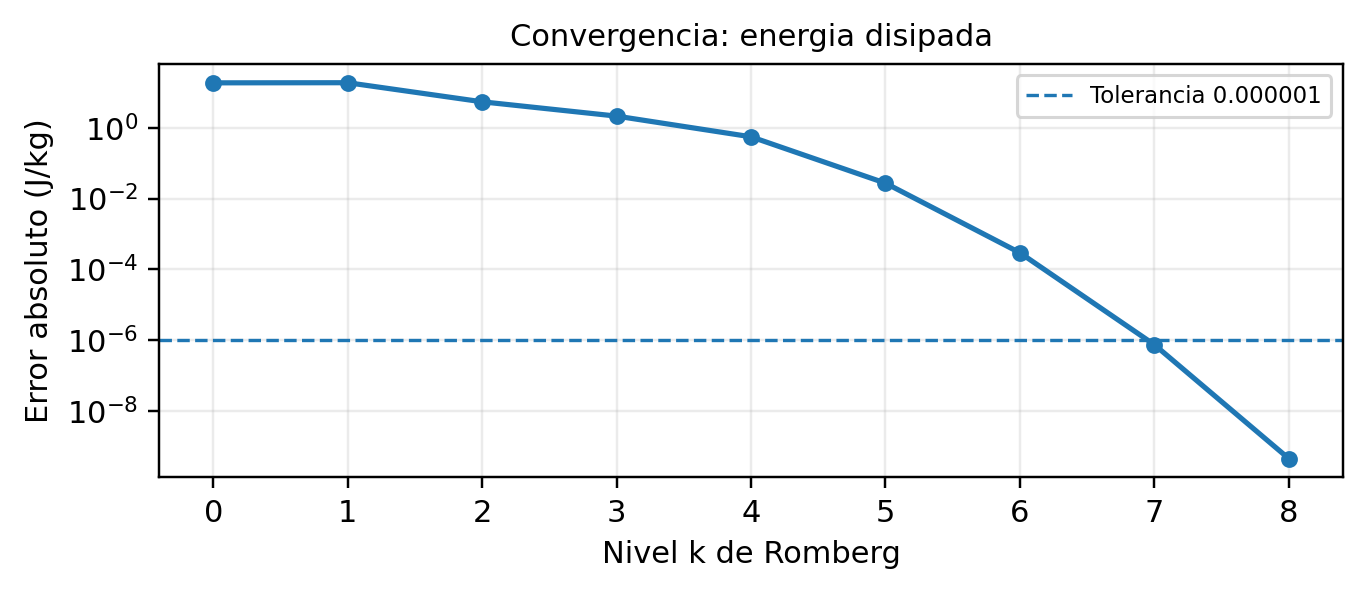
\includegraphics[width=\linewidth]{convergencia_romberg.png}
{\centering\scriptsize Error absoluto de la diagonal de Romberg frente al balance de energía; línea discontinua: $10^{-6}$.\par}
\end{minipage}

\vspace{4pt}
\textbf{4. Obstáculo y decisión de implementación.}
Al revisar los niveles iniciales noté que la malla no resolvía $v^2$: la aproximación $S_{1,1}=0.242788$ J/kg estaba muy lejos de $18.994005$ J/kg. Como los primeros puntos caen cerca de fases de velocidad pequeña, submuestrean las oscilaciones. Para resolverlo refiné la malla, calculando solamente los puntos medios añadidos; así llegué a 257 evaluaciones sin recalcular puntos antiguos. La figura muestra cómo disminuye el error. Esto también evidencia una limitación: una tolerancia aparente en una malla muy gruesa puede no representar el error físico.

\textbf{5. Comparación con Monte Carlo.}
El \emph{mismo} módulo, sin cambios, obtuvo $\pi=3.1415926653$ con 17 evaluaciones y error $1.17\times10^{-8}$. La comparación fue:
\begin{center}
\vspace{-3pt}
{\small\begin{tabular}{@{}lrr@{}}
\toprule
Método para $\pi$ & Evaluaciones & Error\\
\midrule
Romberg & 17 & $1.17\times10^{-8}$\\
Monte Carlo (semilla fija) & $10^6$ & $7.57\times10^{-4}$ (observado)\\
Monte Carlo ($\sigma/\sqrt{N}=10^{-5}$) & $2.70\times10^{10}$ (estimadas) & $10^{-5}$ (típico, no garantizado)\\
\bottomrule
\end{tabular}}
\vspace{-3pt}
\end{center}
Para esa incertidumbre estadística, Monte Carlo requeriría aproximadamente $1.59\times10^9$ veces más evaluaciones; sigue siendo útil en integrales de muchas dimensiones.

\textbf{6. Conclusión.}
Romberg resultó eficiente al refinar suficiente la malla de una función suave; las fórmulas centrales mejoraron al reducir el paso. La validación contra una referencia física y el análisis de errores son necesarios para interpretar resultados numéricos confiables.

\textbf{7. Uso ético de IA.}
Se utilizó ChatGPT como apoyo en programación, depuración, explicación y redacción. Los programas se ejecutaron desde cero y aprobaron sin modificar el verificador original: \textbf{4 de 4 PASS}.

\vspace{3pt}\hrule\vspace{3pt}
{\small\textbf{Código, figura y datos:} \href{https://github.com/cardenascristian-web/fisica-computacional-2026ii/tree/main/Taller_7/taller_oscilador_romberg}{GitHub / Taller\_7 / taller\_oscilador\_romberg} (enlace operativo después de publicar).}
\end{document}
